
  \begin{figure}
    \centering

    \begin{tikzpicture}
      % Root
      \node[draw = black, shape = circle] at (0,0)
      (r) {$0;42$};

      \draw[] (0.7,0.1) rectangle ++(5.8,0.8);
      \onslide<2> {
        \draw[] (0.7,0.1) rectangle ++(5.8,0.8) node[pos=0.5]
        {\texttt{ins(21)}\phantom{, \texttt{ins(64)}, \texttt{del(21)}, ...}};
      }
      \onslide<3> {
        \draw[] (0.7,0.1) rectangle ++(5.8,0.8) node[pos=0.5]
        {\texttt{ins(21)}, \texttt{ins(64)}\phantom{, \texttt{del(21)}, ...}};
      }
      \onslide<4> {
        \draw[] (0.7,0.1) rectangle ++(5.8,0.8) node[pos=0.5]
        {\texttt{ins(21)}, \texttt{ins(64)}, \texttt{del(21)}\phantom{, ...}};
      }
      \onslide<5> {
        \draw[] (0.7,0.1) rectangle ++(5.8,0.8) node[pos=0.5]
        {\texttt{ins(21)}, \texttt{ins(64)}, \texttt{del(21)}, ...};
      }
      \onslide<5-> {
        % HACK: For some reason, when doing this horisontally, we get an
        % unwanted horizontal '|' at the beginning.
        \draw[-|] (3.5,1.3) edge ++(-2.9,0.0);
        \draw[-|] (3.7,1.3) edge node[pos=-0.-0.02, above] {$\tfrac{1}{2} M/B$+} ++(2.9,0.0);
      }
      \onslide<6> {
        \draw[] (0.7,0.1) rectangle ++(5.8,0.8) node[pos=0.5]
        {\texttt{ins(21)}, \texttt{del(21)}, \texttt{ins(64)}, ...};
      }
      \onslide<7> {
        \draw[] (0.7,0.1) rectangle ++(5.8,0.8) node[pos=0.5]
        {\sout{\texttt{ins(21)}}, \sout{\texttt{del(21)}}, \texttt{ins(64)}, ...};
      }
      \onslide<8> {
        \draw[] (0.7,0.1) rectangle ++(5.8,0.8) node[pos=0.5]
        {\sout{\texttt{ins(21)}}, \sout{\texttt{del(21)}}\phantom{, \texttt{ins(64)}, ...}};
      }

      % Left Child
      \node[draw = black, shape = circle] at (-4,-2)
      (c1) {\phantom{0;42}};

      \draw[] (-0.8,-3) -- ++(-2.5,0) -- ++(0,0.8) -- ++(2.5,0);
      \onslide<8-> { \node at (-2.6, -2.6) {...}; }

      % Middle Child
      \node[draw = black, shape = circle] at (0,-2)
      (c2) {\phantom{0;42}};

      \draw[] (3.2,-3) -- ++(-2.5,0) -- ++(0,0.8) -- ++(2.5,0);
      \onslide<8-> { \node at (1.4, -2.6) {...}; }

      % Right Child
      \node[draw = black, shape = circle] at (4,-2)
      (c3) {\phantom{0;42}};

      \draw[] (7.2,-3) -- ++(-2.5,0) -- ++(0,0.8) -- ++(2.5,0);
      % \onslide<-7> { \node at (5.4, -2.6) {...}; }
      \onslide<8-> { \node at (5.9, -2.6) {\texttt{ins(64)}, ...}; }

      % Edges
      \draw[-] (r) edge (c1) edge (c2) edge (c3);
    \end{tikzpicture}
  \end{figure}
